\title{Machine Learning Spring 2019 HW2}
\author{
        Yueh Cheng Liu \\
        National Taiwain University\\
}
\date{\today}
\documentclass[12pt]{article}
\usepackage{amsmath,amssymb}
\usepackage{bbm}
\usepackage{graphicx}
\usepackage{mathtools}
\usepackage{bm}
\DeclareMathOperator{\E}{\mathbb{E}}
\begin{document}
\maketitle

% \begin{abstract}
% This is the paper's abstraasdsadsct \ldots
% \end{abstract}

\section*{1}

$$
\nabla F(A, B)= 
\begin{bmatrix}
    \frac{\delta F(A, B)}{\delta A}  \\
    \frac{\delta F(A, B)}{\delta B} 
\end{bmatrix}
$$

\begin{equation*}
\begin{split}
    \frac{\delta F(A, B)}{\delta A} &= \frac{1}{N} \sum_{n=1}^N \frac{\delta (-y_n(Az_n + B))}{\delta A} \frac{e^{-y_n(Az_n+B)}}{1+ e^{-y_n(Az_n+B)}} \\
    &= \frac{1}{N} \sum_{n=1}^{N} p_n \frac{\delta (-y_n (Az_n + B))}{\delta A} \\
    &= \frac{1}{N} \sum_{n=1}^{N} -p_ny_nz_n
\end{split}
\end{equation*}
and 
\begin{equation*}
\begin{split}
    \frac{\delta F(A, B)}{\delta B} &= \frac{\delta F(A, B)}{\delta B} \\
    &= \frac{1}{N} \sum_{n=1}^{N} \frac{\delta (-y_n (Az_n + B))}{\delta B} \frac{e^{-y_n(Az_n+B)}}{1+ e^{-y_n(Az_n+B)}} \\
    &= \frac{1}{N} \sum_{n=1}^{N} p_n \frac{\delta (-y_n (Az_n + B))}{\delta B} \\
    &= \frac{1}{N} \sum_{n=1}^{N} -p_ny_n
\end{split}
\end{equation*}


\section*{2}

$$
H(F) = 
\begin{bmatrix}
    \frac{\delta^2 F(A, B)}{\delta A^2} & \frac{\delta^2 F(A, B)}{\delta A \delta B} \\
    \frac{\delta^2 F(A, B)}{\delta B \delta A} & \frac{\delta^2 F(A, B)}{\delta B^2}
\end{bmatrix}
$$
\begin{equation*}
\begin{split}
    \frac{\delta \theta(x)}{\delta x} &= \frac{\delta \frac{e^x}{1+e^x}}{\delta x} \\
    &= \frac{\delta (1+e^{-x})^{-1}}{\delta x} \\
    &= -e^{-x} \cdot -(1+e^{-x})^{-2} \\
    &= \frac{1}{1+e^{-x}} \frac{e^-x}{1+e^{-x}} \\
    &= \theta(x) (1 - \theta(x))
\end{split}
\end{equation*}

\begin{equation*}
    \begin{split}
        \frac{\delta^2 F(A, B)}{\delta A^2} &= \frac{ \delta \frac{1}{N} \sum_{n=1}^N -y_nz_n \theta(-y_n(Az_n+B))}{\delta A} \\
        &= \frac{1}{N} \sum_{n=1}^N -y_nz_n \theta(-y_n(Az_n+B)) (1 - \theta(-y_n(Az_n+B))) \frac{\delta (-y_n (Az_n + B))}{\delta A} \\
        &= \frac{1}{N} \sum_{n=1}^N y_n^2z_n^2 \theta(-y_n(Az_n+B)) (1 - \theta(-y_n(Az_n+B))) \\
        &= \frac{1}{N} \sum_{n=1}^N y_n^2z_n^2 p_n (1-p_n)
    \end{split}
\end{equation*}

\begin{equation*}
    \begin{split}
        \frac{\delta^2 F(A, B)}{\delta B^2} &= \frac{ \delta \frac{1}{N} \sum_{n=1}^N -y_n \theta(-y_n(Az_n+B))}{\delta B} \\
        &= \frac{1}{N} \sum_{n=1}^N y_n^2 \theta(-y_n(Az_n+B)) (1 - \theta(-y_n(Az_n+B))) \\
        &= \frac{1}{N} \sum_{n=1}^N y_n^2 p_n (1-p_n)
    \end{split}
\end{equation*}

\begin{equation*}
    \begin{split}
        \frac{\delta^2 F(A, B)}{\delta A \delta B} = \frac{\delta^2 F(A, B)}{\delta B \delta A} &= \frac{ \delta \frac{1}{N} \sum_{n=1}^N -y_nz_n \theta(-y_n(Az_n+B))}{\delta B} \\
        &= \frac{1}{N} \sum_{n=1}^N y_n^2 z_n\theta(-y_n(Az_n+B)) (1 - \theta(-y_n(Az_n+B))) \\
        &= \frac{1}{N} \sum_{n=1}^N y_n^2 z_n p_n (1-p_n)
    \end{split}
\end{equation*}

\section*{3}
$e^{-x} = 0$ when $x\rightarrow\infty$. The target function of soft margin SVM with rbf kernel will be 

$$
\text{min}_\alpha \text{lim}_{\gamma \rightarrow \infty}\frac{1}{2} \sum_{n,m} \alpha_n\alpha_my_ny_me^{-\gamma||x-x'||^2} + \sum_n \alpha_n
= \text{min}_\alpha \sum_n \alpha_n
$$
with constraint $\sum_n y_n \alpha_n = 0$ and $0 \leq \alpha_n \leq C$.

Since the number of postive and negative samples are the same, 
we can choose $\alpha_n = C$ for all $n$ to achieve smallest target function.
The optimal $\bm{\alpha}$ will be all-$C$ vector.
\section*{4}
% \begin{equation*}
%     \begin{split}
%         L_{mse} &= \frac{1}{N} \sum_{n=1}^N (h(x_n) - f(x_n))^2 \\
%         &= \frac{1}{N} \sum_{n=1}^N (w_1x_n + w_0 - x_n + x_n^2)^2 
%     \end{split}
% \end{equation*}
Given $N=2$,
\begin{equation*}
    \begin{split}
        w_1 x_1 + w_0 &= x_1 - x_1^2 \\
        w_1 x_2 + w_0 &= x_2 - x_2^2
    \end{split}
\end{equation*}
Solve $w_0$ and $w_1$ 
\[
    w_1(x_1 - x_2) = (x_1 - x_1^2) - (x_2 - x_2^2)
\]

\[
    w_1 = \frac{(x_1 - x_2) (1-x_1-x_2)}{x_1-x_2} = 1-x_1-x_2
\]

\[
    w_0 = x_1 - x_1^2 - (1 - x_1 - x_2) x_1 = x_1 x_2
\]
Since $x_1, x_2 \in \text{Uinform}(0, 1)$, $\E 1-x_1-x_2 = 0$ and $\E x_1x_2 = 0.25$
\[
    \bar{g}(x) = \E w_1 x + w_0 = 0.25 
\]
\section*{5}

\begin{equation*}
\begin{split}
    (\tilde{y_n} - w^T \tilde{x_n})^2 &= u_n (y_n - w^Tx_n)^2 \\
    &=  (\sqrt{u_n} y_n - \sqrt{u_n}w^Tx_n)^2
\end{split}
\end{equation*}
so that $(\tilde{x_n}, \tilde{y_n}) = (\sqrt{u_n}x_n, \sqrt{u_n}y_n)$

\section*{6}
Let $\epsilon_t$ be the weighted error at step $t$ and $k_t = \sqrt{\frac{1- \epsilon_t}{\epsilon_t}}$. \\
$\epsilon_1 = 0.22$ and $k_1 = \sqrt{\frac{1- \epsilon_1}{\epsilon_1}}$
\begin{equation*}
\begin{split}
    \frac{u_+^{(2)}} {u_-^{(2)}} &= \frac{u_+^{(1)} / k_1 } {u_-^{(1)} * k_1} \\
    &= \frac{1}{k_1^2} = \frac{0.22}{0.78} = 0.282
\end{split}
\end{equation*}

\section*{7}
For integers between $[-M, M]$ has $2M$ interval. $s$ can be $+1$ or $-1$ and $d$ different feature to choose.
Plus the $2$ decision stumps where $g(x)=+1$ and $g(x)=-1$ for all $x$ which are not effected by $d$. 
The number of different decision stump is $2d \cdot 2M+2 = 4dM+2 = 42$. 

\section*{8}
Given $i, s$, there are $|x_i - x_i'|$ number of $\theta$ that makes 
$s \cdot \text{sign}(x_i - \theta) s\cdot \text{sign}(x_i' - \theta) = -1$
and $2M - |x_i - x_i'|$ number of $\theta$ that makes
$s \cdot \text{sign}(x_i - \theta) s\cdot \text{sign}(x_i' - \theta) = +1$.
Combining the result of problem 7,
\begin{equation*}
    \begin{split}
    K_{ds}(x, x') &= 2 + 2 \sum_{i=1}^d (2M - |x_i - x_i'| - |x_i - x_i'|) \\
    &= 2 + 4dM -4\sum_{i=1}^d |x_i - x_i'|
\end{split}
\end{equation*}


\section*{9}
% All E_in [0.3175, 0.3175, 0.32, 0.315, 0.33]
% All E_out [0.36, 0.36, 0.36, 0.4, 0.37]
% 3 50.0 0.315
% 0 0.05 0.36
$\lambda = 50.0$ has the minimum $E_{in} = 0.315$

\section*{10}
$\lambda = 0.05, 0.5, 5$ has the minimum $E_{out} = 0.36$

\section*{11}
% All E_in [0.32, 0.32, 0.3175, 0.31, 0.325]
% All E_out [0.36, 0.36, 0.37, 0.4, 0.37]
% 3 50.0 0.31
% 0 0.05 0.36
$\lambda = 50.0$ has the minimum $E_{in} = 0.31$. 
The result is a little smaller then a single ridge regression.
This is probably because of bagging.

\section*{12}
$\lambda = 0.05, 0.5$ has the minimum $E_{out} = 0.36$.
The result is the same as 10. 
The boostrapping and bagging technique does not help $E_{out}$ in this case.

\section*{13}
\begin{center}
    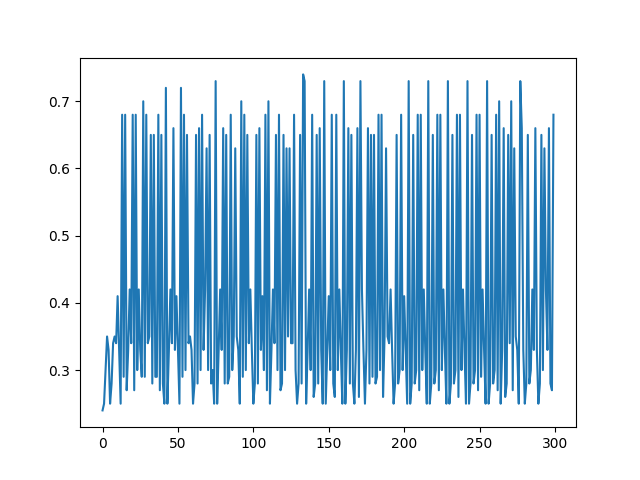
\includegraphics[scale=0.5]{p13.png}
\end{center}
$E_{in}(g_T) = 0.68$. $E_{in}(g_t)$ is low at first. 
After a few steps, the weights of some hard examples (or noises) are larger making the model to fit on those samples.
This increases $E_{in}(g_t)$ and lower the weight of those examples, causing the decrease of $E_{in}(g_{t+1})$.
This repeating routine makes the bouncing curve.

\section*{14}
\begin{center}
    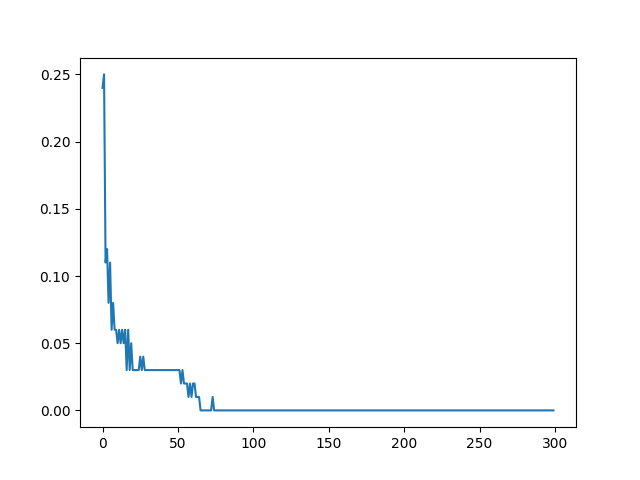
\includegraphics[scale=0.5]{p14.png}
\end{center}
$E_{in}(G_T) = 0$. Following the theoretical guarantee of AdaBoost, $E_{in}(G_t)$ decreases to $0$ fastly.

\section*{15}
\begin{center}
    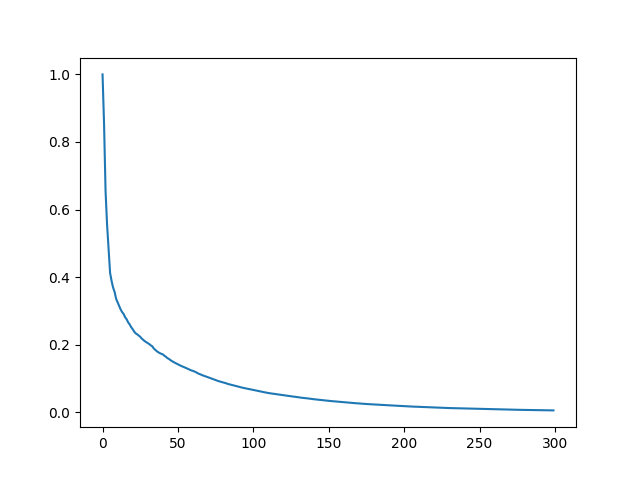
\includegraphics[scale=0.5]{p15.png}
\end{center}
$U_T = 0.0055$. By theoretical prove, $U_t$ will be decreasing and become almost $0$.

\section*{16}
\begin{center}
    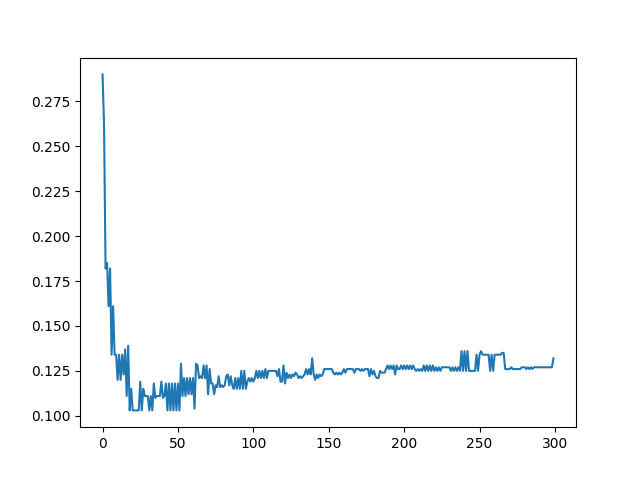
\includegraphics[scale=0.5]{p16.png}
\end{center}
$E_{out}(G_T) = 0.132$. $E_{out}(G_t)$ first decrease to almost $0.1$ 
and then increase a litle due to overfitting.

\section*{17}
\[
    \epsilon_t = \frac{\sum_i u_{t, i} [y_i \neq h_t(x_i)]}{\sum_i u_{t, i}}
    =  \frac{\sum_i u_{t, i}^-}{\sum_i u_{t, i}}
\]
and 
\[
    1 - \epsilon_t = \frac{\sum_i u_{t, i}^+}{\sum_i u_{t, i}}
\]

\begin{equation*}
    \begin{split}
        U_{t+1} &= \sum_i u_{t, i}^+ \sqrt{\frac{\epsilon_t}{1-\epsilon_t}} + \sum_i u_{t, i}^- \sqrt{\frac{1-\epsilon_t}{\epsilon_t}} \\
        &= \sqrt{\epsilon_t(1-\epsilon_t)} (\frac{\sum_i u_{t,i}^+}{1-\epsilon_t} + \frac{\sum_i u_{t,i}^-}{\epsilon_t}) \\
        &= \sqrt{\epsilon_t(1-\epsilon_t)} 2 \sum_i u_{t, i} \\
        &= 2 U_t \sqrt{\epsilon_t(1-\epsilon_t)}
    \end{split}
\end{equation*}

\begin{equation*}
    \begin{split}
        \epsilon (1 - \epsilon) &= - (\epsilon^2 - \epsilon + \frac{1}{4}) + \frac{1}{4} \\
        &= -(\epsilon - \frac{1}{2})^2 + \frac{1}{4}
    \end{split}
\end{equation*}
Thus, $\sqrt{\epsilon(1-\epsilon)}$ will be smaller when $\epsilon$ is a way from $\frac{1}{2}$,
and $\sqrt{\epsilon_t(1-\epsilon_t)} \leq \sqrt{\epsilon(1-\epsilon)}$ since
$\epsilon_t \leq \epsilon < \frac{1}{2}$

\section*{18}


\end{document}


